{
\parskip=10pt
\vspace{8pt}
\hrule

TO: Mr Snowden

In terms of my A2 Computing Project, I have a basic idea which I think would be workable and fit what you described previously, please let me know if you have any more ideas to expand the program.
The program will feature relatively simple visuals, probably 2D, meaning it should run well on low end computers in the school, the program will simulate individual objects at the appropriate level in sped-up real time.
You will be able to set up scenarios by introducing objects, varying the mass and velocity of the object before placement, multiple objects can be placed and they will interact with each other. (n-body problem could be interesting)

Creating the user interface for this will be somewhat of a challenge, likely I will try to integrate it all into a single window as it would remove the need for a secondary library for the user interface, information about what state an object is going to be placed down in (Mass, Velocity, Size, Fixed) As well as simulation state. (Time, Simulation Speed), A right click menu could contain certain options (Presets) but keyboard controls would the primary method of control.

I have also considered implementing a system which would allow the saving and loading of different scenarios, allowing them to be set-up, saved and loaded at other times, which could be useful in a classroom situation, I would be interested to know if you would find this feature useful.

If you have any questions, let me know, I need to have a bit of a dialogue going in order to establish some groundwork, as the project progresses I will have questions for you in regards to particular decisions or compromises that need to be made along the way.

Many Thanks

Byron Theobald.

\vspace{8pt}
\hrule

TO: Byron

A really useful innovation might be to have a graphical way of representing initial velocity, e.g. an arrow extending from each mass, representing the vector for initial velocity.
I like the idea of being able to save the scenario for later on, it would definitely increase the value of the tool.

A very difficult (but very useful) feature might be to be able to tick a box to display both gravitational field lines and lines of equipotential. This is an area of Physics which you haven’t covered yet, but is fairly straightforward...

Thanks for trying a Physics application!

SDS

\vspace{8pt}
\hrule

TO: Mr Snowden

Something I wanted to find out is how you would like the orbital simulator to handle collisions.

Based on my understanding of momentum, simply adding the mass of the two bodies and recalculating the velocity based on conservation of momentum would make sense.

Happy to hear your thoughts on this.

\vspace{8pt}
\hrule

TO: Byron

Yes, provided momentum is conserved, everything will be fine. Remember that they will be 
inelastic collisions (ie KE not conserved).

Your idea below assumes no fragments are ejected - a reasonable assumption to avoid hideous complexity.

Best wishes,
SDS

\vspace{8pt}
\hrule

TO: Mr Snowden

I have attached a copy of the objectives that I will be adheering to during the development and implementation of the current system.

If you could review these and let me know your thoughts.

Many Thanks

Byron Theobald

\vspace{8pt}
\hrule

TO: Byron

All of these look good, nothing that I can think of that isn't on the list.

Best wishes,
SDS

\vspace{8pt}
\hrule

TO: Mr Snowden

I wanted to update you on the current progress of the orbital simulator, apologies for infrequency in that regard.

In its current state the code is sitting at just over 850 lines total.

So far the simulation portion is mostly complete, aside for the implementation of body collision detection and handling.

I have modified the simulation interface to allow it to be completely dynamic, meaning that it is much easier to define as many bodies as necessary in the code. While I have not tested the limits of this, aside from the memory and performance requirements there is no reason why there should be any limit to the number of bodies. (Part of my test plan revolves around benchmarking the performance of large numbers of bodies, up to 64. Back of the envelope calculations suggest that at this number, each frame would take more than 250ms to compute, this is a severe reduction in performance but you are unlikely to need to use more than a few bodies.)

I have also nearly completed the interface to link together the multi-threaded nature of the program, allowing data to seamlessly be transferred between the renderer and the simulation, there is still some parts that need to be added, such as getting new changes made by the user sent to the simulation, ignoring any previously stored simulation data, user changes must take priority.

The next major task is to implement the renderer, this involves some understanding of matrix operations due to the nature of OpenGL programming, however I do not expect this to be a major issue as it is mostly abstracted.

After the renderer is implemented I will then focus on the UI and other utilities.

Attached is an animation of the raw simulation output showing a model sun-planet-moon system

\begin{figure}[H]
  \centering
  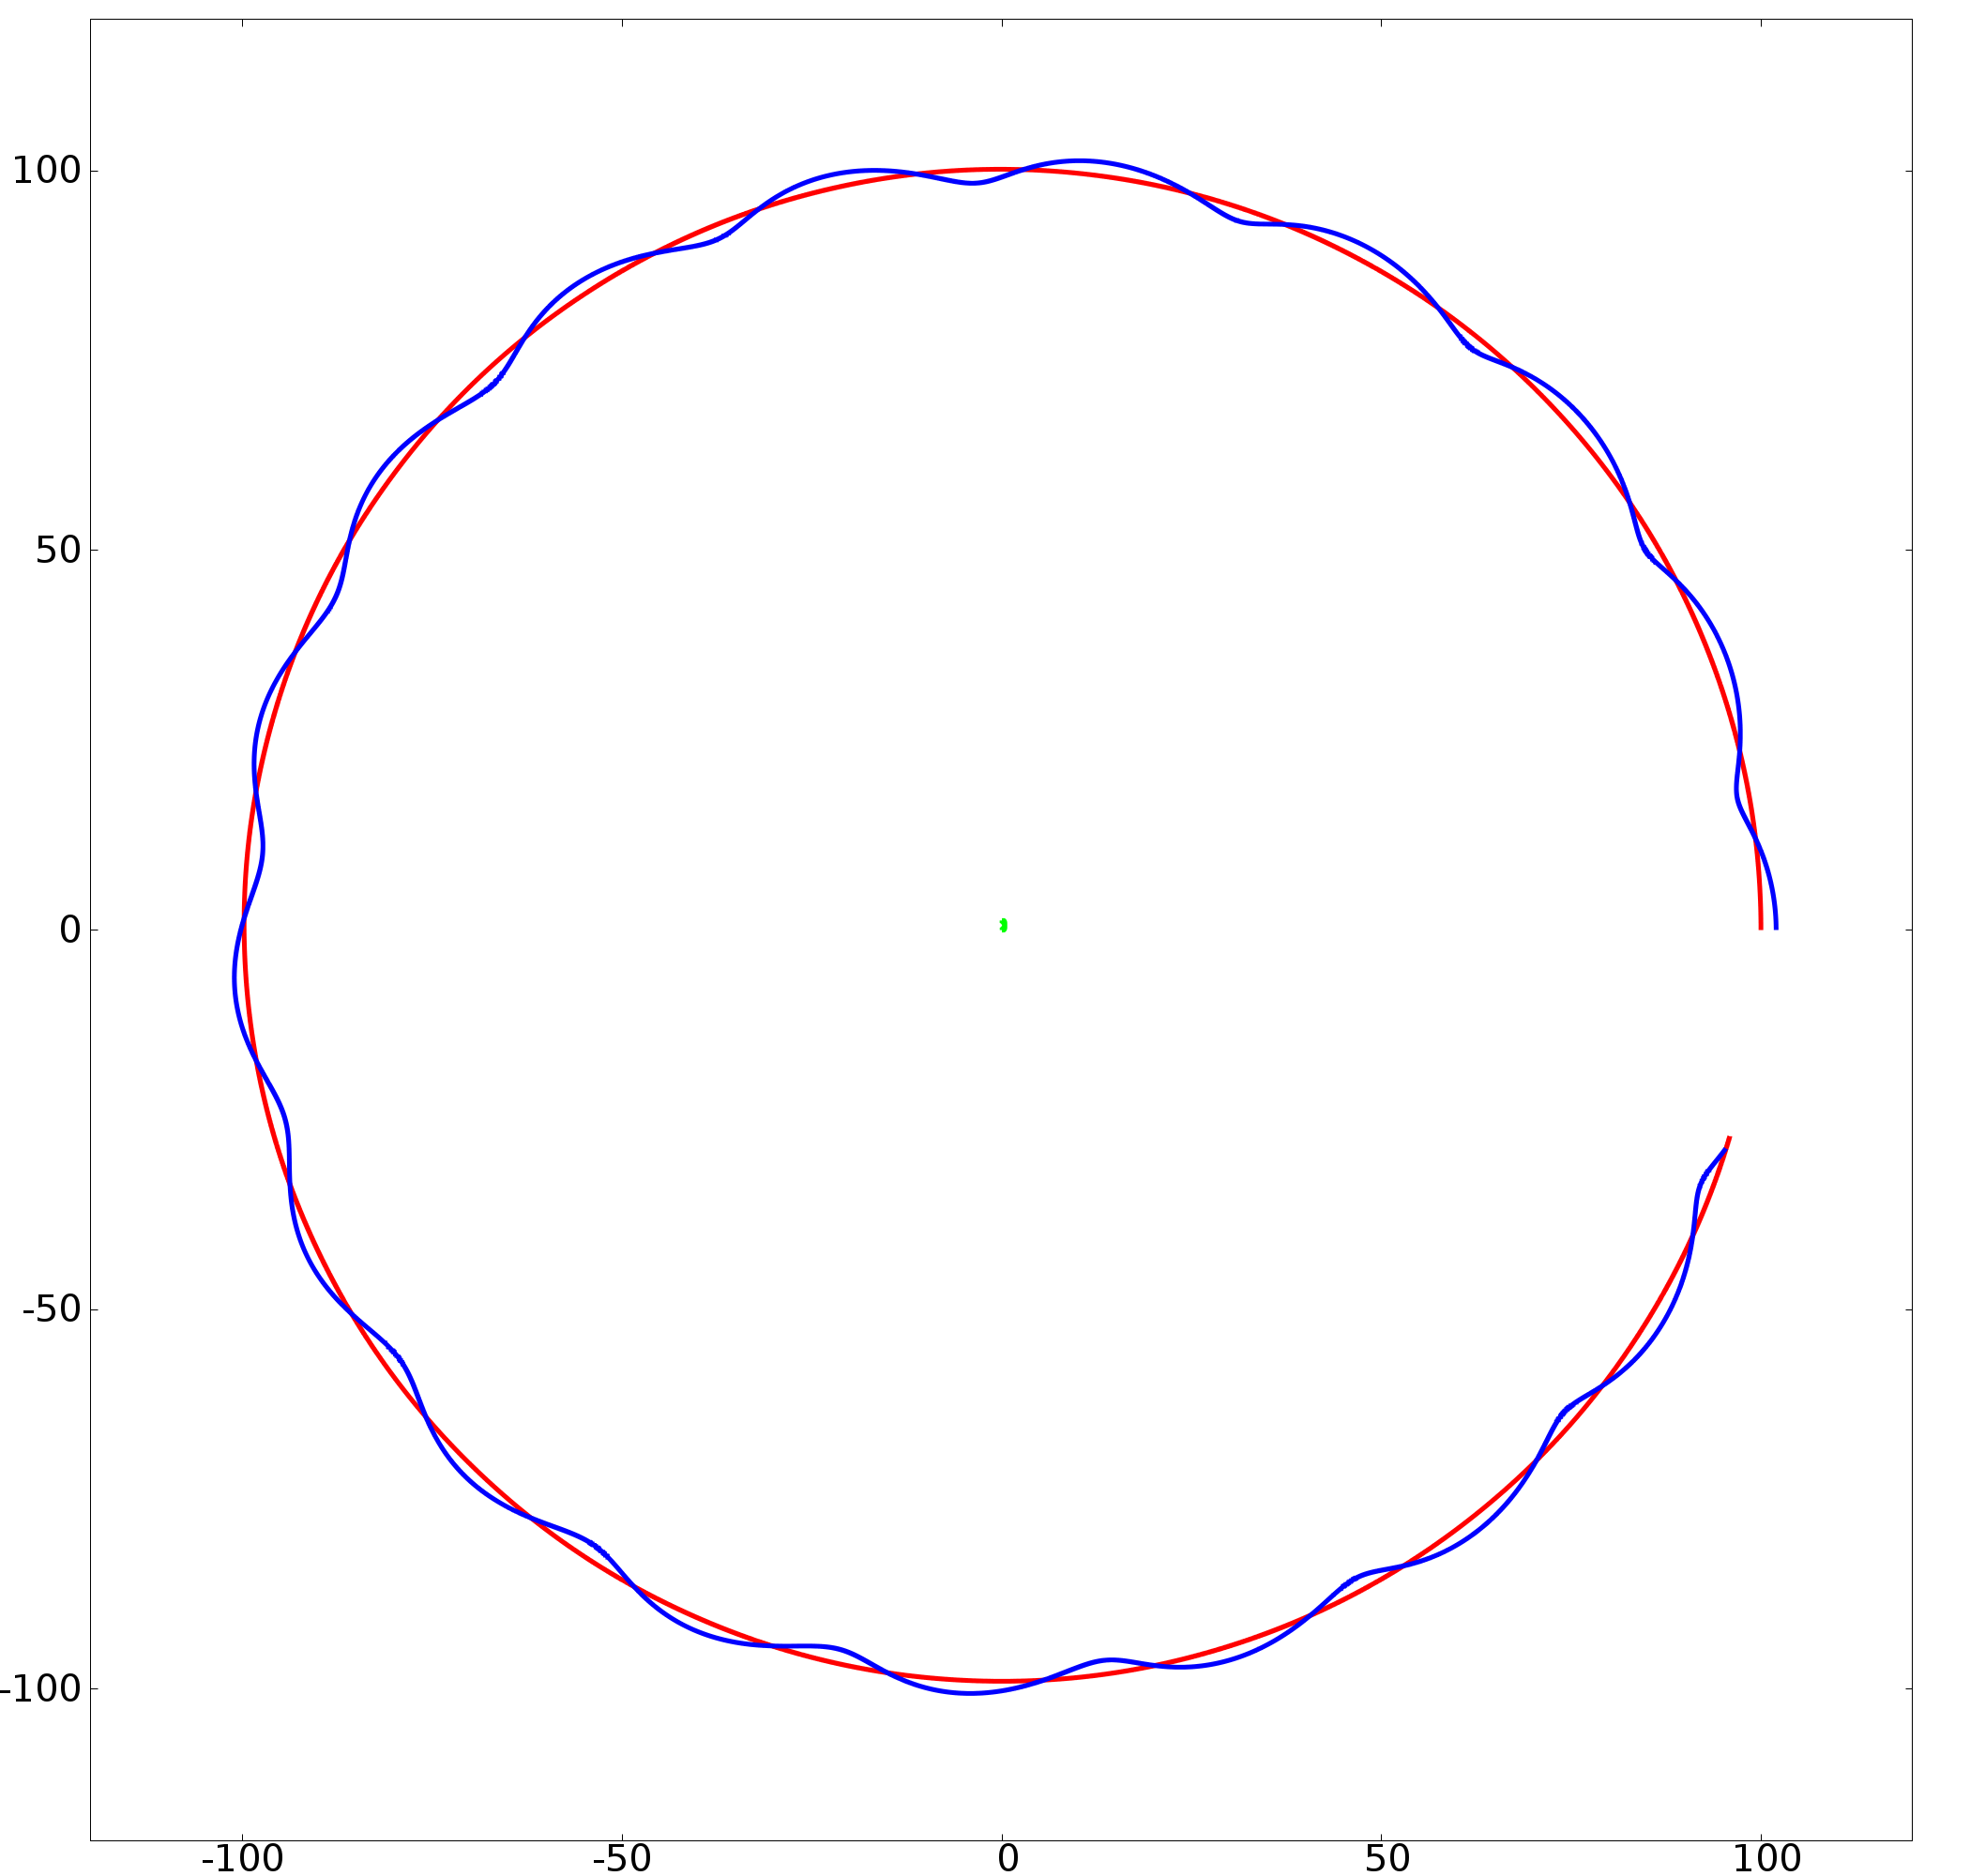
\includegraphics[width=0.6\textwidth]{img/still.png}
  \caption{Three Body Sun-Planet-Moon System}
\end{figure}

\pagebreak
\hrule

TO: Mr Snowden

I implemented a basic version of the rendering module that i will be developing going forward.

Here is a preview:

\begin{figure}[H]
  \centering
  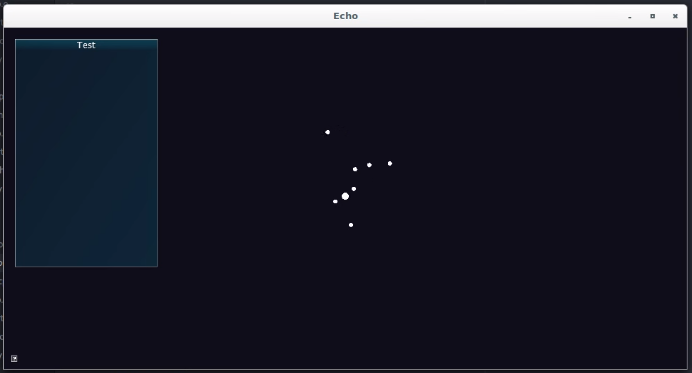
\includegraphics[width=0.9\textwidth]{img/pEcho.png}
  \caption{N-Body Graphics Test}
\end{figure}

Performance is looking extremely promising, will test with a very large number of bodies once I am able to create a distribution system.

\vspace{8pt}
\hrule

TO: Byron

Thanks for the updates. this all looks very promising indeed - keep up the good work and keep me posted!

Best wishes,
SDS

\vspace{8pt}
\hrule

Prototype testing of the simulation showed that it can still support a massive amount of bodies and run smoothly, several orders of magnitude more than expected.

\begin{figure}[!ht]
  \centering
  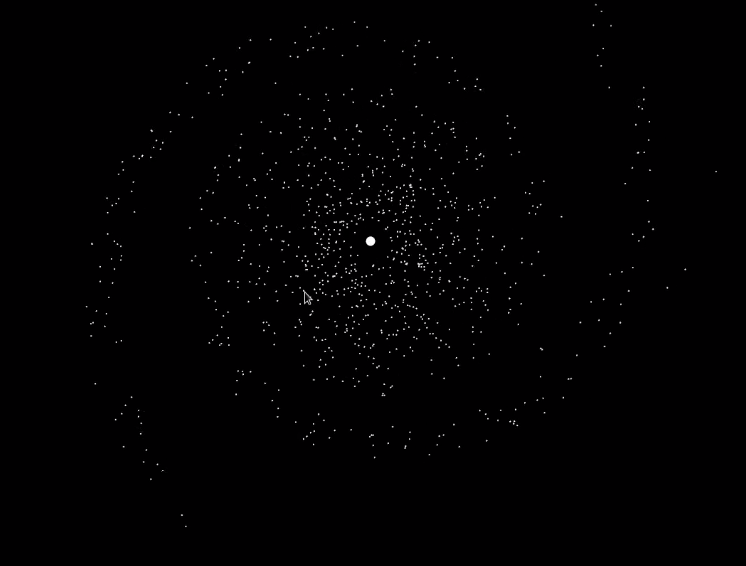
\includegraphics[width=0.9\textwidth]{img/superstructure.png}
  \caption{~1000 Body Superstructure}
\end{figure}

I had a few discussions with Mr Snowden about the potential applications of having large numbers of bodies, I agreed to implement the ability for the user to generate these superstructures; similar to the one shown below, through the interface. 

This could allow the software to be used to simulate a very low body count galaxy collision.

Something that we also decided on was the ability to turn on and off body collisions and combinations, as not having collisions results in the simulation staying more stable for longer.

While the earlier intention was to only consider the simulation for a few bodies, I will now consider the simulation for larger numbers of bodies, the benefit is that if the simulation is correct for 3 bodies, it will be correct for any number.

The other benefit that this brings is the showcase aspect of it, something like this 'looks' really good to anybody who is is studying or considering studying Physics, It is also far more likely to move into the area of inspiration for younger people, increasing their interest in Physics and academia in general. Spectacle is something that can easily affect the way that people think.

\vspace{8pt}
\pagebreak

TO Mr Snowden

As of the week before last I have put a freeze on major programming for the project.

During the weekend (week before last) I decided to rewrite the entire program from scratch, as the way that certain core functions of the program were written made it extremely difficult to add critical user interface controls for adding and deleting bodies, among other things.

I also rewrote major algorithms that stored the forces for each relationship and then summed them on the individual bodies after they had all been calculated, the issue with this is that it was a relatively large memory hog in the program, while it wasn't going to affect its normal use, I still felt that it was worth doing differently.

The current system is now much more efficient, as forces are no longer directly stored in the bodies themselves and instead, each relationship is calculated, converted to acceleration and then summed onto the body object, this is done for both axis and for both bodies in the relationship.

After the full rewrite there where substantial performance gains to the simulation, a 2000 body simulation runs about as well as a 1000 body simulation did previously.

Unfortunately, due to time constraints several features have not been included in the project at this current time, the main omission is the ability to save and load pre-made scenarios.

Regardless of that fact, I feel that in its current state the program is more than usable, I still do need to compile a version that can run on Windows, however that is not priority at the moment.
}